
\chapter{Phase-Scatter Correction of NMR Datasets}

\section{Introduction}

\begin{doublespace}
As previously introduced in \hyperlink{chapter.3}{Chapter 3}, normalization
of data tensors is a commonly performed procedure aimed at minimizing the
within-class variation of two or more groups of observations, relative to
the total or between-class variation in the dataset. Irrespective of whether
separations between classes are obtained using an unsupervised PCA model or a
supervised (O)PLS-DA model, greater statistical significance and increased
biological relevance may be ascribed to separations between classes having
greater variation between groups than within them \cite{worley:abio2013}.
\\\\
Normalization applied directly to hypercomplex NMR data (or its real component)
is sub-optimal, as even small phase differences between observations can
frustrate the estimation of normalization factors
(cf. \hyperlink{section.3.3}{Section 3.3}). Possibly worse, blind
normalization of poorly phased spectral data can accentuate experimentally
irrelevant spectral features in a data tensor during multivariate modeling,
leading the analyst to erroneous conclusions. These difficulties motivated
the development of phase-scatter correction (PSC, \cite{worley:cils2014}) as
a means of simultaneously correcting the coupled phase errors and dilution
errors that are present in hypercomplex NMR data tensors. When hypercomplex
NMR data must be normalized prior to multivariate analyses within the confines
of a metabolomics study, the interrelation of phase and dilution errors is best
handled using phase-scatter correction.
\end{doublespace}

\section{Theory}

\subsection{Multiplicative Scatter Correction}

\begin{doublespace}
Phase-scatter correction (PSC) is effectively an extension of multiplicative
scatter correction (MSC) to handle phase errors during normalization. In MSC,
each real spectrum is scaled around its mean intensity and shifted to match a
reference spectrum, typically the mean of the dataset \cite{fearn:cils2009}.
Optimal normalization factors ($\mathbf{b}$) of a data matrix $\mathbf{X}$ are
determined by a linear regression of the mean-centered reference vector onto
the mean-centered matrix:
\begin{equation}
\big( \mathbf{X} - \langle \mathbf{X} \rangle \big)^T \mathbf{b}
 = \big( \mathbf{r} - \langle \mathbf{r} \rangle \big)^T
\end{equation}
where observations are stored as row vectors in $\mathbf{X}$, and $\mathbf{r}$
is the reference observation row vector. The equation above represents an
overdetermined system of linear equations, therefore the least-squares estimate
of $\mathbf{b}$ may be computed rapidly, and MSC is rather computationally
efficient.
\end{doublespace}

\subsection{Phase-scatter Correction}

\begin{doublespace}
PSC additionally corrects zero- and first-order phase errors during
normalization, requiring a nonlinear optimization of the following objective:
\begin{equation}
Q(\mathbf{X} \mid \mathbf{p})
 = \sum_{n=1}^N \| \mathbf{z}_n \circ \mathbf{x}_n - \mathbf{r} \|_2^2
\end{equation}
where $\circ$ denotes the element-wise product, the mean-centered matrix
$\mathbf{X}$ lies in $\mathbb{H}_1^{N \times K}$, the mean-centered reference
$\mathbf{r}$ lies in $\mathbb{H}_1^K$, and the set of parameters $\mathbf{p}$
includes a normalization factor and two phase errors per observation
in $\mathbf{X}$:
\begin{equation}
\mathbf{p} = \{
  b_1, \dots b_N,
  \theta_{0,1}, \dots \theta_{0,N},
  \theta_{1,1}, \dots \theta_{1,N} \}
\end{equation}
and each vector $\mathbf{z}_n$ contains the normalization and phase corrections
for the $n$-th observation $\mathbf{x}_n$:
\begin{equation}
z_{n,k} = b_n e^{u_1 (\theta_{0,n} + \theta_{1,n} k)}
\end{equation}

Because the reference observation $\mathbf{r}$ is fixed during optimization,
minimization of $Q(\mathbf{X} \mid \mathbf{p})$ may be achieved by
independently minimizing each observation's contributions. Minimization is
carried out for every observation in the data matrix using Levenberg-Marquardt
nonlinear least squares \cite{marquardt:jsiam1963} as implemented by the
{\it leasqr} function in GNU Octave, a function similar to MATLAB's
{\it nlinfit}. Each corrected spectrum $\hat{\mathbf{x}}_n$ is then returned
from optimization as follows:
\begin{equation}
\hat{\mathbf{x}}_n
 = \mathbf{z}_n \circ \mathbf{x}_n
 + \langle \mathbf{r} \rangle
\end{equation}

Phase-scatter correction of 50 1D \hnmr{} NMR spectra having 32,768 complex
points each requires approximately 30 seconds on a single-core 3.2 GHz Intel
workstation running GNU Octave 3.6.
\end{doublespace}

\subsection{Ensemble Phase Correction}

\begin{doublespace}
It is important recognize that the phase-scatter correction objective function
$Q(\mathbf{X} \mid \mathbf{p})$ provides no measure of ideal phase values,
meaning that PSC requires an additional phase correction step prior to its
execution in order to ensure adequate initial conditions. Even when
$\mathbf{X}$ has been suitably phase-corrected, PSC may still attempt to
minimize scatter between spectra by re-introducing phase errors. This
undesirable behavior of PSC may be observed when large disparities in
spectral intensities are present between observations. To correct this,
a standard phase correction objective
$f : \mathbb{H}_D^{K} \to \mathbb{R}$ may be combined with
the PSC objective using a Lagrange multiplier, like so:
\begin{equation}
\Lambda(\mathbf{X} \mid \mathbf{p}) =
 -\sum_{n=1}^N f(\boldsymbol{\theta}_n \circ \mathbf{x}_n) +
 \lambda \sum_{n=1}^N \| \mathbf{z}_n \circ \mathbf{x}_n -
            \langle \mathbf{Z} \circ \mathbf{X} \rangle \|_2^2
\end{equation}
where the correction matrix $\mathbf{Z}$ has the same form as in PSC, expressed
as a real diagonal matrix of normalization factors $\mathbf{B}$ and a
hypercomplex matrix of phase factors $\mathbf{\Theta}$:
\begin{equation}
\mathbf{Z} = \mathbf{B} \mathbf{\Theta}
\end{equation}
and $\boldsymbol{\theta}_n$ is the $n$-th row of $\mathbf{\Theta}$. The new
ensemble phase correction (EPC) objective function
$\Lambda(\mathbf{X} \mid \mathbf{p})$ balances the potentially opposing goals
of phase correction and scatter correction through the Lagrange multiplier
$\lambda$, and does not require the specification of a reference observation
$\mathbf{r}$. In effect, EPC allows its scatter correction reference to float
as the current mean of the data, $\langle \mathbf{Z} \circ \mathbf{X} \rangle$.
This floating reference requires the simultaneous optimization of all the
parameters in $\mathbf{p}$, unlike phase-scatter correction. Efficient
minimization of $\Lambda(\mathbf{X} \mid \mathbf{p})$ may be accomplished by
a modified Nelder-Mead simplex optimization procedure \cite{nelder:compj1964},
which serially updates the simplices of all observations at each global
iteration and maintains the current mean vector
$\langle \mathbf{Z} \circ \mathbf{X} \rangle$ at each update.
\\\\
In contrast to phase-scatter correction, which seeks to minimize the scatter
of data matrix observations around a fixed reference, ensemble phase correction
approaches the dilemma of entwined phase and normalization errors from an
opposing direction by introducing a scatter term into a standard automatic
phase correction procedure. The amount of normalization achieved by EPC is
directly controlled by the magnitude of $\lambda$: in the opposite limits of
$\lambda = 0$ and $\lambda \to \infty$, EPC becomes equivalent to standard
phase correction and phase-scatter correction with a floating reference,
respectively.
\end{doublespace}

\section{Materials and Methods}

\begin{SCfigure}
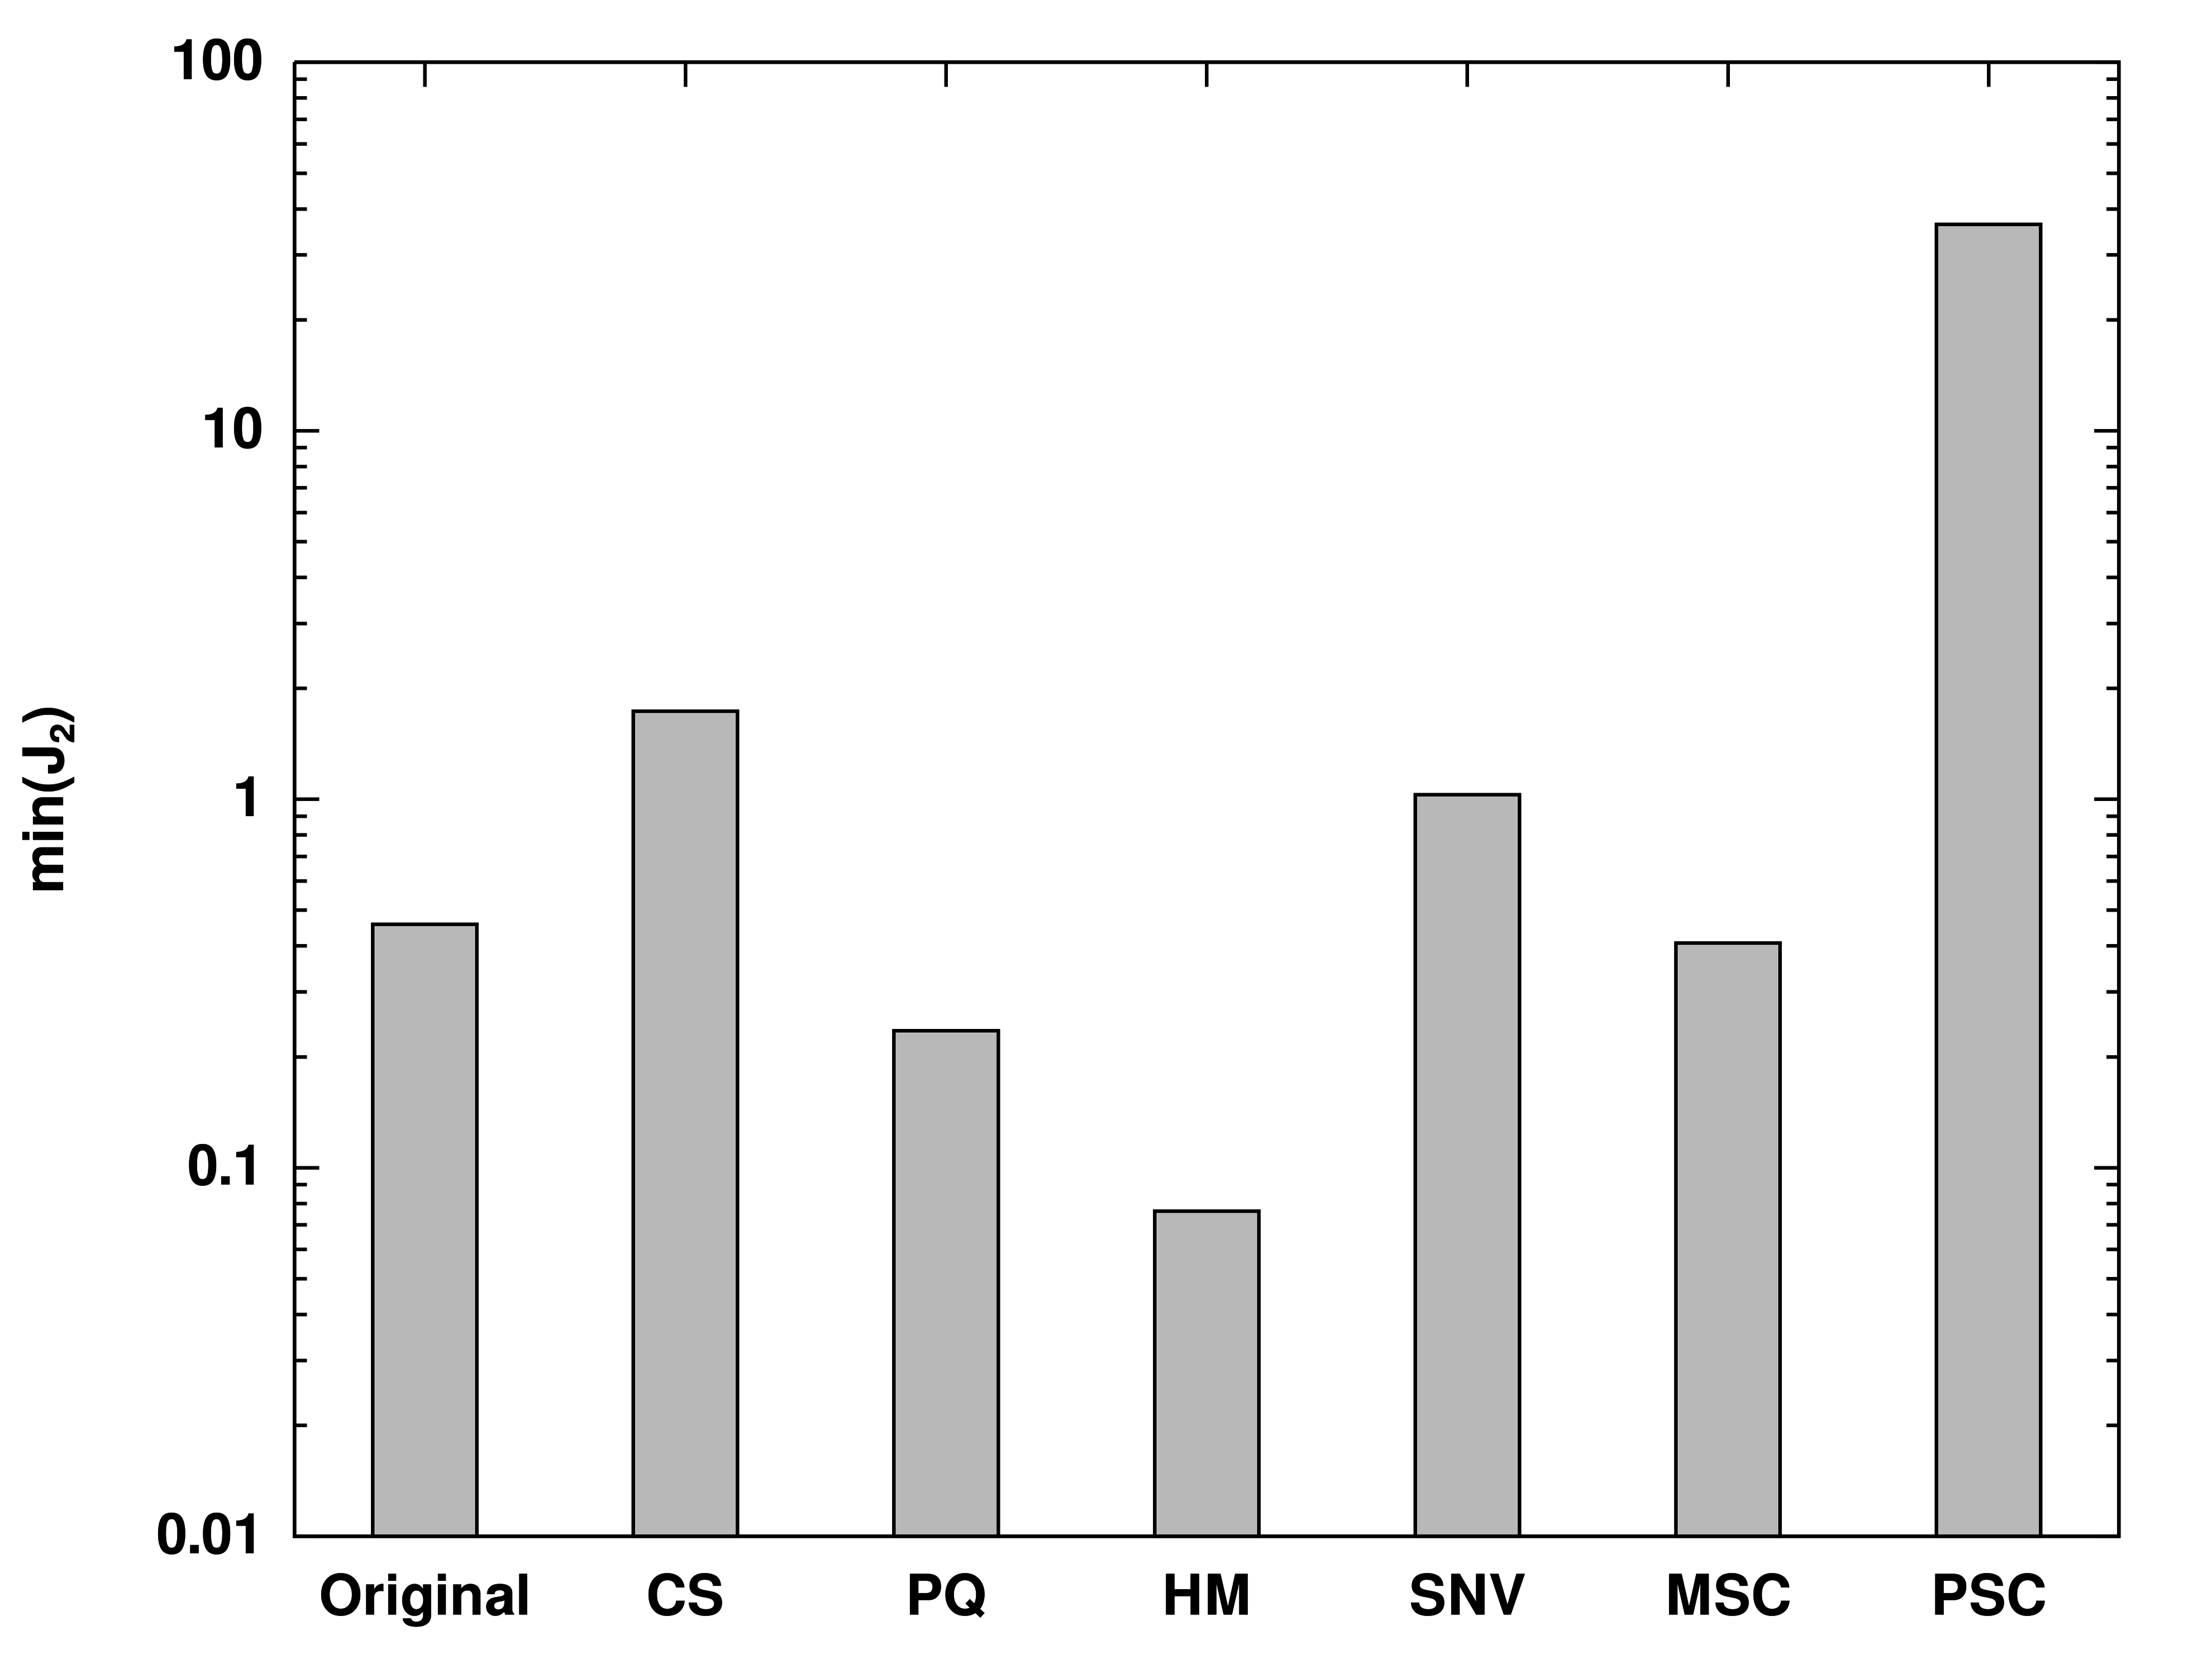
\includegraphics[width=3.25in]{figs/pscorr/01-minj2.png}
\caption
      [Cluster Quality after Normalization and PCA Modeling.]{
  {\bf Cluster Quality after Normalization and PCA Modeling.}
  \\
  Comparison of PCA cluster quality for \hnmr{} NMR metabolomics data
  normalized using different algorithms. The minimum $J_2$ value (worst
  cluster quality) for each model is reported here, as it is a more effective
  indicator of overall model and cluster quality than the mean or median.
}
\label{figure.6.1}
\end{SCfigure}

\subsection{NMR Data Processing}

\begin{doublespace}
Previously collected \hnmr{} NMR spectral data from published work
\cite{halouska:acscb2012} was leveraged as a typical metabolomics dataset
for performance analysis of PSC versus other normalization methods. Free
induction decays were loaded into GNU Octave 3.6 \cite{eaton2008} for
processing using MVAPACK routines \cite{worley:acscb2014}. Time-domain signals
were zero-filled to 32,768 points and Fourier transformed, resulting in
a complex data matrix of 177 spectra divided amongst 16 classes
($N$ = 177, $K$ = 32,768, $M$ = 16). Spectra were both automatically phase
corrected by simplex entropy minimization \cite{chen:jmr2002} and manually
phase corrected by applying a constant phase shift to all spectra. Both
automatically and manually phase corrected datasets were then normalized using
the CS, PQ, HM, SNV, MSC and PSC methods
(cf. \hyperlink{subsection.3.4.3}{Chapter 3}).
Each normalized data matrix was binned using a uniform 0.04 ppm bin width,
scaled per-variable to unit variance, and subjected to PCA. The $J_2$ statistic
\cite{koutroumbas2006} was calculated for each class to provide a measure of
cluster quality for the PCA scores from each normalization method, as follows:
\begin{equation}
J_{2,m} = \frac{|\mathbf{C}|}{|\mathbf{C}_m|}
\end{equation}
where $\mathbf{C}_m$ is the covariance matrix of the scores in class $m$,
$\mathbf{C}$ is the covariance matrix of all scores, and the vertical bars
represent the matrix determinant. Thus, as a cluster shrinks relative to the
entirety of the scores-space data, its $J_2$ statistic will increase. While
$J_2$ provides a measure of individual cluster tightness, it does not capture
the degree of cluster overlap within a dataset. \figref{6.1}{Figures 6.1} and
\figref{6.2}{6.2} show the results of the $J_2$ calculation for normalization
methods applied to real \hnmr{} NMR metabolomics data.
\end{doublespace}

\begin{SCfigure}
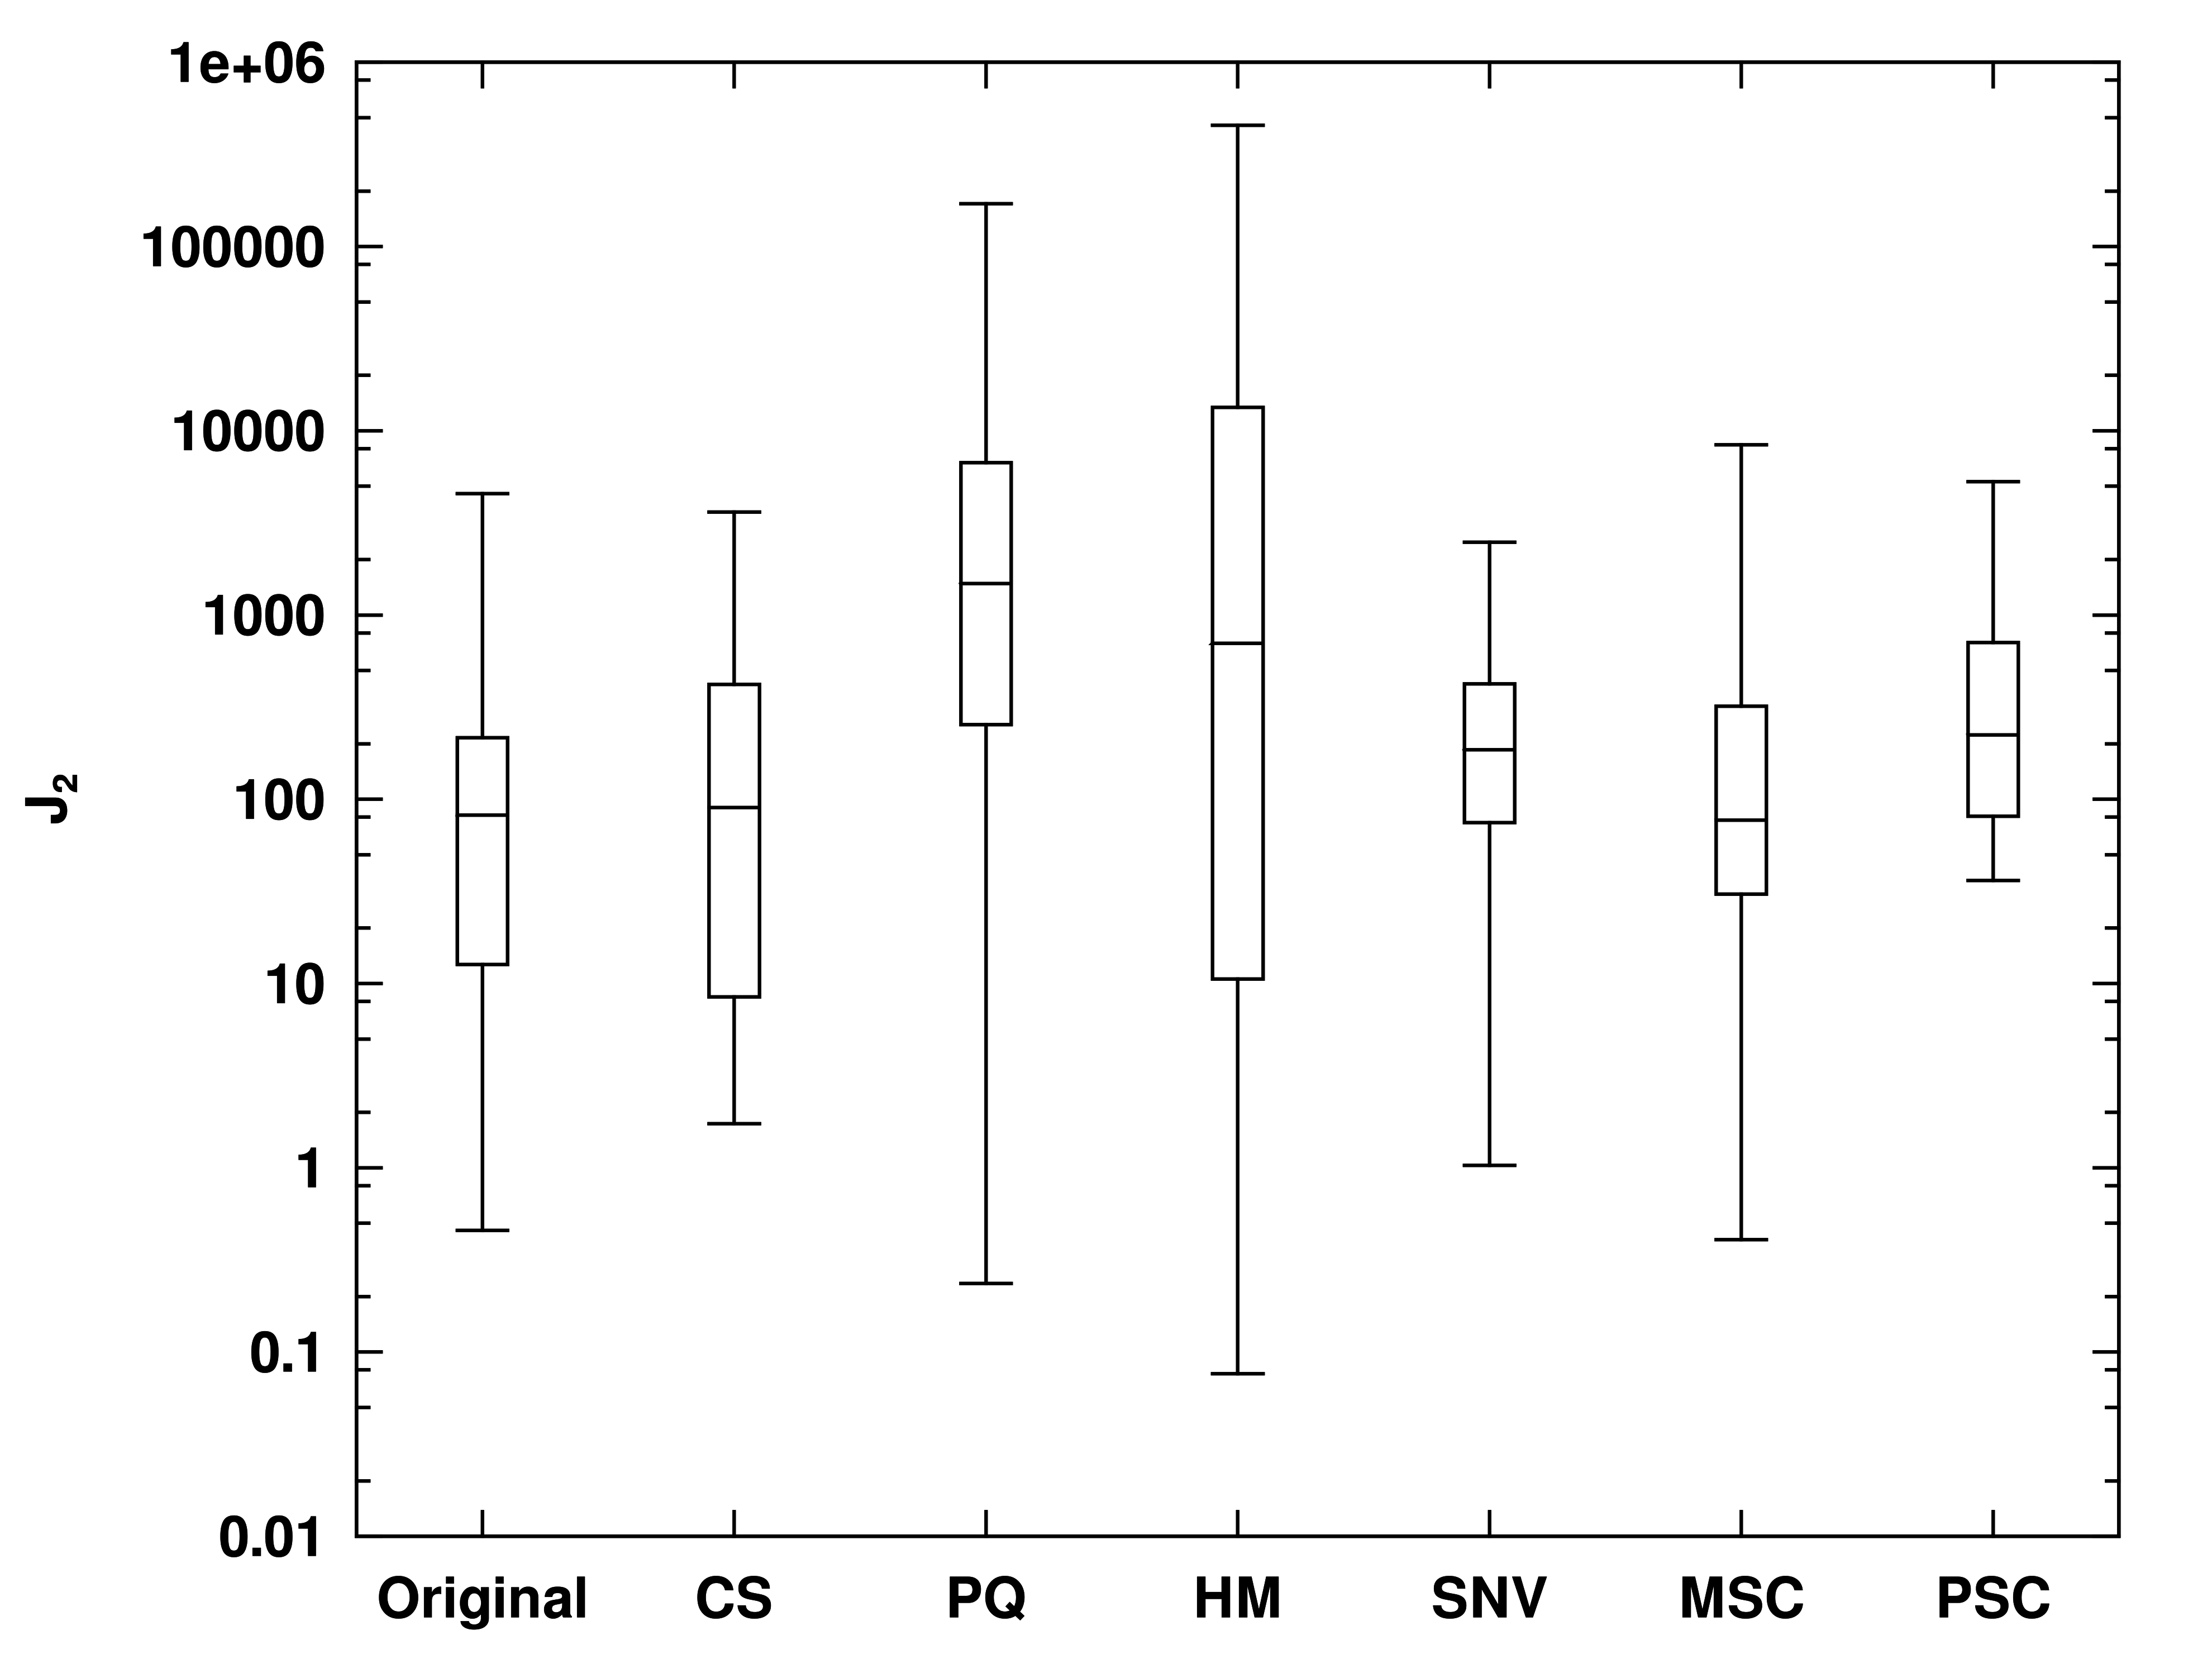
\includegraphics[width=3.25in]{figs/pscorr/02-allj2.png}
\caption
      [Cluster Quality after Normalization and PCA Modeling.]{
  {\bf Cluster Quality after Normalization and PCA Modeling.}
  \\
  Comparison of PCA cluster quality for \hnmr{} NMR metabolomics data
  normalized using different algorithms. For each normalization method, a
  box is defined by the estimated first and third quartiles of $J_2$ for the
  clusters and whiskers are defined by the range of the $J_2$ values for the
  clusters. For this dataset, the minimum $J_2$ value is most instructive,
  given the fact that overall model quality is not well-reflected by the
  $J_2$ metric in the case of distorted principal components.
}
\label{figure.6.2}
\end{SCfigure}

\begin{doublespace}
To quantify differences between extracted principal components of automatically
and manually phase corrected datasets, the angle between the first principal
component loading vector of each pair of models ($\varphi$) was calculated as
follows:
\begin{equation}
\varphi = \cos^{-1}\left( {\mathbf{p}_{auto}}^T \mathbf{p}_{man} \right)
\end{equation}
where $\mathbf{p}_{auto}$ and $\mathbf{p}_{man}$ are the first-component
loadings computed from a given normalization method's data after automatic
and manual phase correction, respectively. The loading angle $\varphi$ for a
given normalization method is a reflection on that method's ability to properly
normalize data and produce consistent PCA models from different initial phase
error conditions.
\end{doublespace}

\begin{table}[h!]
\caption{Metabolite Spectra Used in Monte Carlo Simulations.}
\begin{center}
\begin{tabular}{l l l l}
  \hline
  Aminobutyrate & Adenosine & Alanine     & Arginine   \\
  Asparagine    & Aspartate & Choline     & Citrulline \\
  Ethanolamine  & Fructose  & Galactose   & Glucose    \\
  Glutamate     & Glutamine & Glycine     & Histidine  \\
  Isoleucine    & Lactate   & Leucine     & Lysine     \\
  Malate        & Maltose   & Myoinositol & Ornithine  \\
  Phenylalanine & Proline   & Putrescine  & Serine     \\
  Succinate     & Sucrose   & Threonine   & Valine
\end{tabular}
\end{center}
\end{table}

\subsection{Simulated NMR Datasets}

\begin{doublespace}
The \hnmr{} NMR spectra of 100 mM samples of 32 metabolites (Table 6.1) at
pH 7.4 were downloaded from the Biological Magnetic Resonance Bank
(BMRB, \cite{ulrich:nar2008}) and fit to mixtures of complex Lorentzian
functions using ACD/1D NMR Processing (Advanced Chemistry Development).
Peak amplitudes ($A$), chemical shifts ($\omega_0$), and widths ($\lambda$)
returned from fitting were loaded into GNU Octave to generate simulated spectra
having 65,536 data points and a spectral width of 11 ppm, centered at
4.7 ppm, based on the following model function:
\begin{equation}
s(\omega_k) =
 \sum_{p=1}^P
 \frac{A_p \lambda_p}
      {\lambda_p + u_1 (\omega_k - \omega_{0,p})}
\end{equation}
where $s(\omega_k)$ is the $k$-th data point of the spectrum, $P$ equals the
number of peaks, and $u_1$ equals the imaginary unit. Spectra were referenced
and normalized to the DSS peak, and peaks corresponding to HOD and DSS were
subsequently removed, resulting in a basis set of 32 perfectly-phased,
noise-free metabolite spectra. Finally, the basis metabolite spectra were
stored row-wise in a matrix $\mathbf{S}$ for later use in Monte Carlo
calculations.
\end{doublespace}

\begin{figure}[ht!]
\includegraphics[width=6in]{figs/pscorr/03-rmse.png}
\caption
      [Monte Carlo Normalization Results.]{
  {\bf Monte Carlo Normalization Results.}
  \\
  Results of 100 Monte Carlo iterations at 0.2$^\circ$ zero-order phase error,
  indicating the ability of all normalization methods to recover the true
  dilution factor of a nearly perfectly phased dataset. Red points reflect the
  dilution factors calculated by integrated the DSS peak and blue points
  reflect the dilution factor estimates from normalization. Upper panels show
  the dilution factors recovered from automatically phased data after
  normalization, and lower panels show dilution factors recovered from
  unphased data after normalization.
}
\label{figure.6.3}
\end{figure}

\subsection{Monte Carlo Experiments}

\begin{doublespace}
Using the basis metabolite spectra, a dataset of 48 simulated metabolomics
spectra ($\mathbf{X} \in \mathbb{H}_1^{N \times K}$) was generated according
to the following equation:
\begin{equation}
\mathbf{X}
 = \mathbf{A} \left( \mathbf{C} \mathbf{S} + \mathbf{1} \mathbf{r}^T \right)
 + \mathbf{E}
\end{equation}
where $\mathbf{A} \in \mathbb{R}^{N \times N}$ is a diagonal matrix of dilution
factors $\alpha_n$, $\mathbf{C} \in \mathbb{R}^{N \times P}$ is a matrix of
metabolite concentrations, $\mathbf{S} \in \mathbb{H}_1^{P \times K}$ is the
previously created metabolite basis set, $\mathbf{r} \in \mathbb{H}_1^K$ is a
spectrum of the DSS reference peak, $\mathbf{1} \in \mathbb{R}^N$ is a vector
of ones, and $\mathbf{E} \in \mathbb{H}_1^{N \times K}$ is a matrix of complex
Gaussian white noise. Dilution factors were drawn from a log-normal
distribution having zero mean and $\sigma = 0.25$. Concentrations in
$\mathbf{C}$ were drawn from normal distributions with parameters chosen to
mimic those in Torgrip et al. (Table 6.2) \cite{torgrip:metab2008}. The
resultant data in $\mathbf{X}$ is a simulated set of $N = 48$ metabolite
extracts, spiked with 100 $\mu$M DSS, where six distinct classes arise from
differences in the concentrations of alanine, asparagine, glutamate, malate,
proline, sucrose and valine. All other metabolites were assigned concentrations
from a normal distribution having $\mu = 5$ $\mu$M and $\sigma = 0.5$ $\mu$M.
\end{doublespace}

\begin{table}[h!]
\caption{Metabolite Concentrations Altered in Monte Carlo Simulations.}
\begin{center}
\begin{tabular}{l | l l l l l l}
  \hline
  {\bf Metabolite} & $\mathbf{C_A}$ ($\mu$M) & $\mathbf{C_B}$ ($\mu$M) &
                     $\mathbf{C_C}$ ($\mu$M) & $\mathbf{C_D}$ ($\mu$M) &
                     $\mathbf{C_E}$ ($\mu$M) & $\mathbf{C_F}$ ($\mu$M) \\
  \hline
  Alanine    &  $9.2 \pm 1.4$    &  $19.6 \pm 1.6$    &  $16.9 \pm 1.2$  &
                $6.5 \pm 0.66$   &  $26.2 \pm 3.6$    &  $13.5 \pm 1.1$  \\
  Asparagine &  $6.8 \pm 0.86$   &  $11.7 \pm 1.8$    &  $19.0 \pm 1.9$  &
               $14.7 \pm 1.2$    &  $24.8 \pm 2.6$    &  $17.4 \pm 1.0$  \\
  Glutamate  & $13.3 \pm 1.7$    &   $9.2 \pm 1.5$    &  $18.8 \pm 1.9$  &
               $16.9 \pm 2.1$    &  $25.0 \pm 3.5$    &   $6.9 \pm 1.0$  \\
  Malate     & $14.2 \pm 1.2$    &  $11.9 \pm 1.4$    &  $22.0 \pm 5.1$  &
                $6.7 \pm 0.68$   &   $9.4 \pm 0.72$   &  $18.0 \pm 2.4$  \\
  Proline    & $11.4 \pm 1.5$    &  $18.4 \pm 3.1$    &  $14.7 \pm 2.4$  &
                $6.9 \pm 0.62$   &   $9.8 \pm 1.5$    &  $23.7 \pm 2.9$  \\
  Sucrose    &  $7.1 \pm 0.9$    &  $17.2 \pm 2.1$    &  $19.3 \pm 2.0$  &
               $13.2 \pm 1.9$    &   $9.3 \pm 0.56$   &  $23.3 \pm 2.7$  \\
  Valine     &  $9.0 \pm 0.85$   &  $26.3 \pm 2.3$    &  $13.4 \pm 1.2$  &
               $20.4 \pm 1.7$    &   $6.7 \pm 0.90$   &  $17.0 \pm 1.5$  \\
\end{tabular}
\end{center}
\end{table}

\begin{doublespace}
Monte Carlo simulations were run to assess the performance of all discussed
normalization methods over various amounts of phase error added to
$\mathbf{X}$. Forty-six phase error points were calculated, in which the
standard deviation of $\theta_0$ was linearly increased from $0^\circ$ to
$5^\circ$. The standard deviation of $\theta_1$ at each point was equal to
one tenth that of $\theta_0$. Both $\theta_0$ and $\theta_1$ were assigned
zero mean. For each phase error point, 100 Monte Carlo iterations were
performed with different sets of random dilution factors. Spectra in the
de-phased $\mathbf{X}$ matrix were automatically phase corrected using simplex
entropy minimization and normalized each time using CS, PQ, HM, SNV, MSC and
PSC methods. Normalization to unit DSS integral was also performed for
reference. An identical set of normalization calculations was performed on the
unphased data. Estimated dilution factors were compared to the true values
to produce a root-mean-square dilution error, $RMSE(\alpha)$, for each method.
\figref{6.3}{Figure 6.3} shows the $RMSE(\alpha)$ result of Monte Carlo
simulation at $0.2^\circ$ phase error. To assess normalization effects on
multivariate model quality, spectra from each method were uniformly binned
with 0.04 ppm bin widths, each bin scaled to unit variance, and subjected
to PCA. Values of $J_2$ for each of the six classes were then calculated,
and the median of the values was reported for each Monte Carlo iteration.
The $\varphi$ values between automatically phased and unphased principal
component loadings were also calculated at each iteration to asses each
normalization method's ability to produce consistent models in the presence
of phase errors. \figref{6.4}{Figure 6.4} summarizes the results of Monte
Carlo simulation over all phase errors based on $RMSE(\alpha)$, $J_2$
and $\varphi$.
\end{doublespace}

\begin{figure}[ht!]
\includegraphics[width=6in]{figs/pscorr/04-montecarlo.png}
\caption
      [Summary of Monte Carlo Simulation Results.]{
  {\bf Summary of Monte Carlo Simulation Results.}
  \\
  Results of the Monte Carlo simulation over all phase error points.
  ({\bf A}) As phase error increases, dilution factor estimates from all
  methods except PQ remain fairly stable. Estimates from PSC compete with
  MSC, but suffer in comparison with HM.
  ({\bf B}) However, $J_2$ values indicate that PSC outperforms all other
  normalization methods at producing tight clusters at any realistic
  phase error.
  ({\bf C}) Finally, values of $\varphi$ calculated from PCA loadings indicate
  that PSC maintains the highest model consistency in the face of imperfectly
  phased data. Phase error on the $x$-axis refers to zero-order error; it
  should be noted that each point also contains first-order phase error as
  discussed in the Methods.
}
\label{figure.6.4}
\end{figure}

\section{Results}

\begin{doublespace}
On the real metabolomics spectral data, PSC normalization resulted in the
highest quality clusters (\figref{6.5}{Figure 6.5}) according to the $J_2$
statistic shown in \figref{6.1}{Figure 6.1}. Given the fact that the spectra
were each automatically phase corrected before any normalization was applied,
this observed increase in $J_2$ must be due to the correction of subtle phase
differences \emph{between} spectra not detectable by correcting each spectrum
individually. It is important to note that, while PQ and HM produce higher
median $J_2$ values (\figref{6.2}{Figure 6.2}), this is an artifact of large
distortions of their respective PCA loadings, and not always reflective of
higher-quality clusters. Because $J_2$ is a per-cluster statistic, it is
only an ideal measure of overall scores-space model quality when all
clusters are nearly identically distributed. Models containing highly
distorted components may contain several high-quality clusters and a
few extremely low-quality clusters, resulting in a high mean or
median $J_2$ value. For that reason, the lower bound of $J_2$ for
each method -- effectively the worst cluster quality -- was chosen as a better
indicator of overall model quality than the median. In fact, PSC produced the
most consistent model loadings between automatically and manually phase
corrected data, with a $\varphi$ value of 14.5$^\circ$. This can be compared to
$\varphi$ values of 89.6$^\circ$ and 20.2$^\circ$ for PQ and HM, respectively.
\\\\
Moreover, Monte Carlo analysis of PSC versus contemporary normalization methods
show that PSC offers a unique advantage during multivariate analysis. Results
of Monte Carlo normalization after automatic phase correction and summarized
in \figref{6.4}{Figure 6.4}, and scatter plots of recovered dilution factors
are shown in \figref{6.3}{Figure 6.3}. While PSC fails to recover true
dilution factors as accurately as DSS, CS or HM normalization, it does
remain competitive with MSC at all phase errors (\figref{6.4}{Figure 6.4A}).
PSC normalization yields tighter clusters than all other methods, as is
apparent from \figref{6.4}{Figure 6.4B}. Furthermore, PSC results in
dramatically lower values of $\varphi$ than all other methods, indicating that
residual phase errors left uncorrected by automatic phase correction are
significant enough to distort principal component loadings when normalized by
any method other than PSC (\figref{6.4}{Figure 6.4C}).
\end{doublespace}

\begin{figure}[ht!]
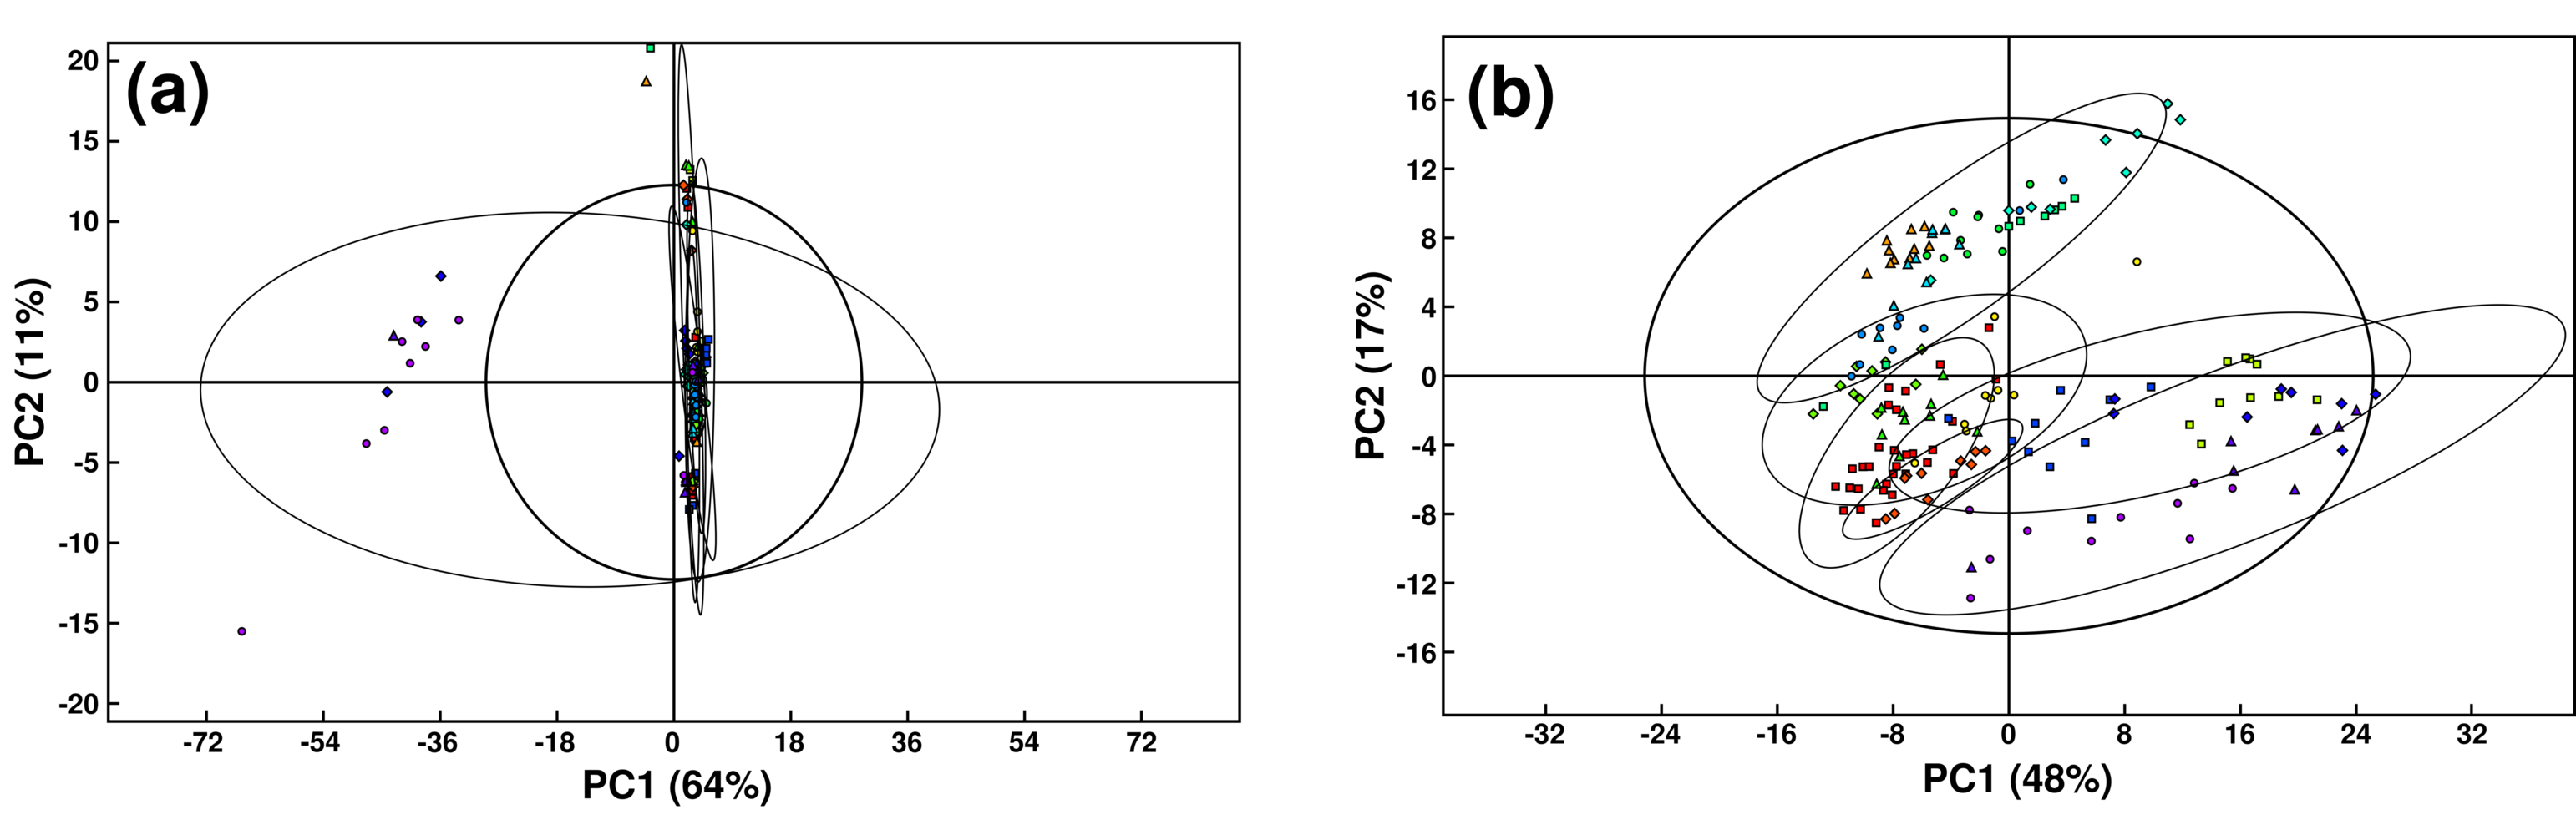
\includegraphics[width=6in]{figs/pscorr/05-scores.png}
\caption
      [Distortion of Principal Components by PQ Normalization.]{
  {\bf Distortion of Principal Components by PQ Normalization.}
  \\
  PCA scores of a typical metabolomics dataset after automatic phasing
  followed by either PQ or PSC normalization. In both plots, ellipses denote
  different classes of antibiotic treatment of \emph{Mycobacterium smegmatis}
  and differing symbols within each ellipse represent different antibiotic
  subclasses.
  ({\bf A}) PQ normalization amplifies residual phase differences left behind
  after automatic phasing, but ({\bf B}) PSC normalization produces a more
  interpretable PCA model by correcting residual phase differences.
}
\label{figure.6.5}
\end{figure}

\section{Discussion}

\begin{doublespace}
As is evident from visual inspection of both the real metabolomics dataset and
the Monte Carlo simulated datasets, correction of minute phase differences
between spectra yields a substantial improvement in cluster quality in
multivariate analyses. In general, phase differences contribute significantly
to spectral lineshape difference in \hnmr{} NMR data. This effect is especially
pronounced in the case of PSC normalization of spectra containing significant
and consistent broad background signals, where normalization alone cannot
comparably standardize baselines (cf. \hyperlink{chapter.7}{Chapter 7}).
\\\\
One particularly striking result of the Monte Carlo simulations is the
difference between automatically phase corrected and unphased dilution factor
estimates (\figref{6.3}{Figure 6.3}). In fact, examination of dilution factors
estimated by DSS integration clearly shows that automatic phase correction
introduces variation into the dataset through minute differences
in $\theta_0$ and $\theta_1$ between spectra. This artificial variation
is then amplified through normalization, as is especially apparent in the
case of PQ normalization.
\\\\
In their report on HM normalization, Torgrip et al. noticed the potential
unsuitability of the explained sum of squares (\rsqx{}) for assessing model
quality differences due to normalization methods \cite{torgrip:metab2008}.
As a ratio measure, explained sum of squares is not suitable for comparing
the qualities of PCA models trained on different data, or any preprocessing
done prior to building the models \cite{kjeldahl:jchemo2010}. Therefore, the
$J_2$ statistic was chosen as an alternative means of comparing cluster quality
during Monte Carlo simulation. Effectively, $J_2$ measures the ratio of the
area of a cluster in scores space relative to the total scores-space area,
regardless of how much variation the model captures. Even still, because $J_2$
is a per-cluster statistic, it is not an ideal measure of overall scores-space
model quality, especially for models containing highly distorted components.
Mean or median $J_2$ values of a model may be high in this case, despite the
fact that the model scores are useless from the perspective of class
discrimination. Thus, the minimum $J_2$ was chosen as a more effective
indicator of overall cluster quality.
\end{doublespace}

\section{Conclusions}

\begin{doublespace}
Phase-scatter correction is a novel algorithm for simultaneously correcting
zero- and first-order phase errors and random dilution factors in \hnmr{}
NMR chemometric data. While PSC only performs comparably to MSC in dilution
factor estimation, it more consistently yields high-quality clusters and
interpretable models when used prior to PCA decomposition. PSC can be fully
automated through prior automatic phase correction of the dataset, has no
tunable parameters, and makes no assumptions regarding line shape, baseline
flatness, or intensity distributions in the data. These qualities lend PSC to
use in chemometrics as a new method of normalizing NMR data entering into
multivariate analyses such as PCA or PLS. The latest implementation of PSC
is available in the MVAPACK toolbox \cite{worley:acscb2014}.
\end{doublespace}

\bibliographystyle{abbrv}
\bibliography{bworley}

